\documentclass[10pt,letterpaper,twoside]{article}
\usepackage{code/manuscript_assets/researchpreprint}
\usepackage{amsmath,amssymb,amsthm,booktabs,graphicx}
\usepackage[hidelinks]{hyperref}
\newcommand{\norm}[1]{\left\lVert#1\right\rVert}
\newtheorem{theorem}{Theorem}
\begin{document}
\title{Fast Hamming Product-Kernel Transfer for Surface-Code Syndrome Probabilities}
\author{Molena Huynh}\email{molena.huynh@jmp.com}
\affiliation{North Carolina State University}
\maketitle

\begin{abstract}
Transferring decoder probabilities across physical fault rates requires a
representation that respects the binary geometry of syndrome histories. An
equal-class-prior Hamming product kernel is studied on the complete public
distance-three archive associated with a cryogenic decoder. The kernel table
is applied by one two-point transform per syndrome bit, reducing a dense
$2^b\times2^b$ kernel multiplication to $O(b2^b)$ arithmetic and $O(2^b)$
storage. A normalization theorem bounds probability error from class-score
errors. History width and kernel bandwidth are selected by rolling rate
holdout; the two highest physical fault rates, comprising twenty million
simulated shots, remain untouched. On this confirmation set the product kernel
has log loss 0.2871, versus 0.5358 for a hierarchical blend, 0.6333 for tuned
logistic regression, and 0.6931 for a constant predictor. Exact lookup has
higher balanced accuracy, 0.9189 versus 0.9038, but substantially worse log
loss, 0.7724. Thus the supported improvement concerns calibrated probability
transfer rather than every classification metric. A separate hierarchical
operator audit confirms decreasing storage and approximation error. Optimized
dense multiplication is faster through 1024 records, whereas the hierarchy
crosses over at 2048 records on the recorded platform. The contribution
is the exact binary-cube kernel algorithm and its authenticated transfer
evaluation, not a hardware decoder or a hierarchical speedup.
\end{abstract}

\section{Authenticated transfer task}

The source is Zenodo record 11166209, version 1.0.1, under CC BY 4.0
~\cite{Yon2024}. Seven CSV files summarize ten million Stim-generated
shots each at increasing physical fault rates. Every row contains a binary
$4\times4$ syndrome history, a logical label, and its shot multiplicity. The
archive has 75,598 rows representing 70 million shots. It is an authenticated
simulation record, not quantum-hardware data.

Rates indexed 0--4 form training and rolling development cohorts. Rates 5 and
6, with physical fault rates 0.005 and 0.010, form the fixed confirmation set.
All metrics use equal total weight for the two logical classes while retaining
within-class shot multiplicities. The model therefore estimates an
equal-class-prior conditional probability, matching balanced accuracy rather
than the archive class prevalence. Table~\ref{tab:data} records the resulting
source and holdout contract.

\begin{table}[t]
\caption{Data and locked transfer protocol.}
\label{tab:data}
\begin{ruledtabular}\begin{tabular}{lr}
Quantity & Value\\ \hline
Syndrome bits $b$ & 16\\
Source rows & 75,598\\
Represented shots & 70,000,000\\
Development rates & indices 2--4\\
Confirmation rates & 0.005, 0.010\\
Confirmation shots & 20,000,000\\
Selected history width & 2 cohorts
\end{tabular}\end{ruledtabular}
\end{table}

\section{Binary-cube product kernel}

Encode a syndrome as $s\in\{0,1\}^b$. For bandwidth $0\le\rho\le1$, set
\begin{equation}
 K_\rho(s,t)=\rho^{d_H(s,t)}.
\end{equation}
For class $c$, let $q_c(t)$ be normalized weighted counts in the selected
history window. Scores and probabilities are
\begin{equation}
 a_c(s)=\sum_tK_\rho(s,t)q_c(t),\qquad
 p(s)=\frac{a_1(s)}{a_0(s)+a_1(s)}. \label{eq:probability}
\end{equation}
The registered grid contains history widths 1--4 and logarithmically spaced
bandwidths including $\rho=0$. Each development rate is predicted only from
lower-rate cohorts. The selected pair is refitted on the two cohorts ending at
rate index four.

\begin{theorem}[Tensor factorization and transform cost]
\label{thm:fwht}
In lexicographic binary order,
\begin{equation}
 K_\rho=\begin{bmatrix}1&\rho\\\rho&1\end{bmatrix}^{\otimes b}.
\end{equation}
Both class-score tables can be computed in $2b2^b$ pair updates, using
$O(2^b)$ working storage per class, without forming $K_\rho$.
\end{theorem}
\begin{proof}
The Hamming distance is additive over coordinates, hence
$\rho^{d_H(s,t)}=\prod_{j=1}^b\rho^{\mathbf1\{s_j\ne t_j\}}$.
The factor for bit $j$ equals the displayed two-by-two matrix entry, proving
the Kronecker identity. Applying one factor updates every disjoint pair of
table entries, requiring $2^b$ scalar-output updates per bit and class.
In-place pair updates store only the current score table.
\end{proof}

\begin{theorem}[Probability perturbation]
\label{thm:normalization}
Let $a_0,a_1\ge0$, $d=a_0+a_1>0$, and suppose
$|\widetilde a_c-a_c|\le\varepsilon_c$ with
$\varepsilon_0+\varepsilon_1<d$. Then
\begin{equation}
 \left|\frac{\widetilde a_1}{\widetilde a_0+\widetilde a_1}
 -\frac{a_1}{d}\right|
 \le\frac{a_0\varepsilon_1+a_1\varepsilon_0}
 {d(d-\varepsilon_0-\varepsilon_1)}. \label{eq:normbound}
\end{equation}
\end{theorem}
\begin{proof}
Writing $\delta_c=\widetilde a_c-a_c$ and clearing denominators gives
\begin{equation}
 \widetilde p-p=\frac{a_0\delta_1-a_1\delta_0}
 {d(d+\delta_0+\delta_1)}.
\end{equation}
The numerator is at most $a_0\varepsilon_1+a_1\varepsilon_0$ in magnitude,
and the second denominator factor is at least
$d-\varepsilon_0-\varepsilon_1$.
\end{proof}

\section{Confirmation results}

Table~\ref{tab:results} separates probability calibration from thresholded
classification. The Hamming kernel has the lowest log loss. Exact lookup has
the highest balanced accuracy and lowest Brier score, but its near-zero
probabilities are severely penalized when an unseen-rate label contradicts
the lookup. The transform therefore improves the primary probabilistic metric
without dominating every metric.

\begin{table}[t]
\caption{Class-balanced confirmation metrics over the two held-out rates.}
\label{tab:results}
\begin{ruledtabular}\begin{tabular}{lrrr}
Method & Log loss & Brier & Bal. acc.\\ \hline
Constant & .6931 & .2500 & .5000\\
Logistic & .6333 & .1299 & .8412\\
Exact lookup & .7724 & \textbf{.0715} & \textbf{.9189}\\
Hamming kernel & \textbf{.2871} & .0767 & .9038\\
Hierarchy blend & .5358 & .1294 & .8410
\end{tabular}\end{ruledtabular}
\end{table}

\begin{figure}[t]
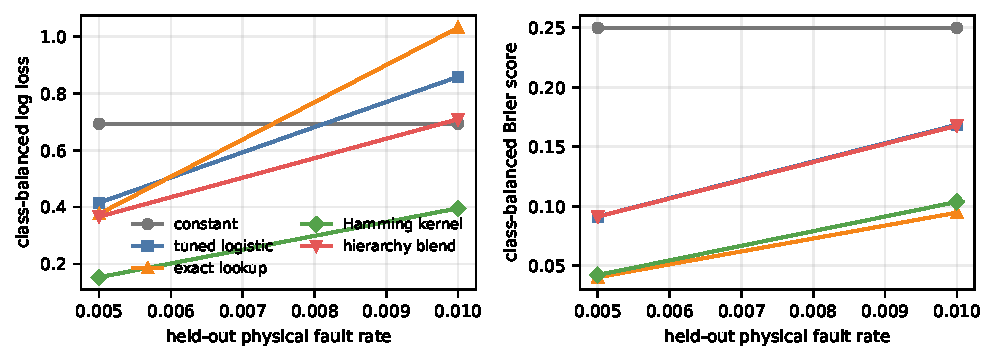
\includegraphics[width=\columnwidth]{code/results/figures/fig_rate_audit.pdf}
\caption{Rate-resolved log loss and Brier score on both confirmation cohorts.
The product kernel retains the log-loss advantage as the fault rate doubles.}
\label{fig:rates}
\end{figure}

At fault rate 0.005, kernel log loss is 0.1527 and balanced accuracy is 0.9464.
At 0.010 the values are 0.3955 and 0.8707. Figure~\ref{fig:rates} shows the
degradation directly rather than merging the two regimes into one favorable
number.

\section{Representation audit}

A hierarchical approximation is not needed by the $b=16$ product kernel: the
exact tensor transform already has linear-in-$b$ table complexity. The prior
hierarchical route is retained as a negative control. On authenticated subsets
of 256--2048 rows, its relative output error decreases from
$2.09\times10^{-5}$ to $3.53\times10^{-6}$ and stored fraction decreases from
0.219 to 0.039. Optimized dense application is faster through 1024 records,
whereas the hierarchy is faster at 2048 records on the recorded platform;
Fig.~\ref{fig:runtime} reports the complete crossover without extrapolation.

\begin{figure}[t]
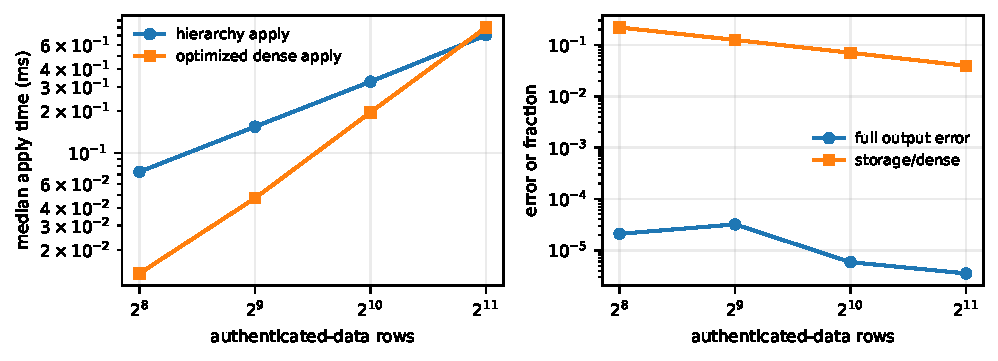
\includegraphics[width=\columnwidth]{code/results/figures/fig_runtime_audit.pdf}
\caption{Measured hierarchy and dense-apply time, together with approximation
error and storage fraction. The compressed representation saves storage and
crosses the dense timing only at the largest tested size.}
\label{fig:runtime}
\end{figure}

\section{Scope}

The experiment tests rate transfer on simulated distance-three syndromes.
It does not measure threshold behavior, hardware drift, decoding latency, or
larger code distances. Exact lookup remains preferable when thresholded
accuracy alone determines the objective. The product-kernel contribution is
narrower: rolling-selected Hamming smoothing supplies substantially better
held-out probability calibration, an exact $O(b2^b)$ transform, and a
conditioning bound for approximate class scores. All rate deterioration and
the negative hierarchical timing result remain part of the evidence.

\bibliographystyle{plainnat}
\bibliography{code/manuscript_assets/references}
\end{document}
